\chapter{竞价云实例上分布式服务的可用性与成本模型}
\label{cha:jupiter}

\section{本章概述}
\label{sec:jupiter_intro}
云计算的出现大大提升了计算资源的使用率。云租户通过租用计算资源避免了自行搭建及维护本地集群的大量软件、硬件、人力成本,同时根据自身计算需求可以方便地动态调整计算资源用量。云平台提供商通过聚合大量的云租户的计算资源使用需求,提升了计算资源的使用率。由于底层集群基础设施的运行和维护成本相对固定,提升计算资源使用率可以为云平台带来更好的收益。为了进一步提升资源使用率,Amazon EC2 近年来推出了拥有新的计费方式的竞价云实例。Amazon EC2对于这种新型计算实例的介绍如下:``竞价云实例向用户提供了为所需的 Amazon EC2 云计算资源设定价格的方式。用户只需简单地对空闲的 Amazon EC2 竞价云实例给出竞价,只要竞价不低于该实例的市场价格即可马上运行、使用该竞价云实例。竞价云实例节点的市场价格则是根据供需关系不断变化的。''从云平台提供者的角度看,该举措能继续提升空闲计算资源的使用率。对于云租户来说,竞价云实例更加便宜能够大大节省成本实现经济计算。然而,正如云平台对竞价云实例节点的介绍所述,竞价云实例不能被认为是一直可用的。无论实际环境中底层硬件的可用性如何,竞价云实例都可能因竞价低于该类型节点的市场价格而被云平台回收导致不可用。这对部署在竞价云实例节点上的分布式服务的可用性分析是一个新的挑战。

在分布式计算中,一些基础的服务被认为必须是高可用(High Availability)的。分布式锁服务是一个常见的例子。作为许多分布式应用的基础组件,分布式锁服务必须一直处于可用状态。任何锁服务的失效将导致整个分布式系统的无法运行。另一个例子是分布式存储服务,一个提供数据存储的基础组件。这些服务通常被认为是十分关键的,应该尽可能可靠。它们不同于可以在失效真正发生后进行修复的批处理任务\cite{5975137, Yi:2010:RCS:1844768.1845343}。对于一些关键服务,安全性必须在任何时候首先得以保证,如:一个互斥锁不能分配给超过一个申请者。这样的服务通常都有它们自身的容错机制,如:基于Paxos的状态机复制机制(State Machine Replication)。只要系统中的大多数节点在足够长的一段时间内可用,这些被应用的算法在保证正确性的同时能够保证进展性(不发生活锁,设定的目标最终达成)。

既然基于Paxos的容错机制可以容忍一个分布式服务中任何非大多数的节点失效,能否通过用竞价云实例节点替换原有按需云实例节点来提供同样高可用的分布式服务呢?用同样数量(或是更多)的竞价云实例节点替换一个分布式系统中的按需云实例节点非常简单,但分析这样一个分布式系统是否能提供同之前按需云实例节点同样可用性级别的服务以及其实际的可用性则不是那么容易。新型竞价云实例节点特有的竞价不足失效(out-of-bid failure)让分布式服务的可用性分析变得十分复杂。同传统分布式系统模型不同,节点失效概率不再是一个很小的常数。因此,传统的用可容忍失效节点数来标明分布式系统可用性级别的方式需要通过概率失效模型加以修正。

综上,使用竞价云实例节点提供分布式服务同时保证和使用按需云实例节点相同的可用性级别是一个新的挑战。本章先提出了基于竞价云实例节点的分布式系统可用性的形式化模型,然后基于该模型提出了一个针对此类分布式服务的竞价框架。该竞价框架能够根据竞价云实例节点市场价格变化自动给出竞价决策以保证设定的系统可用性级别,同时节省分布式服务的成本。

使用易错的竞价云实例节点构建高可用的分布式服务是可以实现的。可以将高可用分布式服务构建在分别属于不同可用区的竞价云实例上,这保证了分布式服务中的各个节点的失效概率是独立同分布的。这种跨地理区域的多副本配置广泛用于高可用分布式服务中,如: Google 的 Spanner \cite{Corbett:2012:SGG:2387880.2387905},Amazon 的 Dynamo \cite{DeCandia:2007:DAH:1294261.1294281},以及Microsoft 的 Windows Azure Storage\cite{Calder:2011:WAS:2043556.2043571}。以分布式锁服务为例,使用5个物理隔离的Amazon EC2按需云实例构建的一个分布式锁服务在一个月内的故障停机时间一般少于30秒。\footnote{根据Amazon EC2的Service Level Agreement(SLA),按需云实例的可用性不会低于99\%,否则使用者将获得相当于付费30\%的赔偿。由于来自不同的地理位置,5个按需云实例是失效独立的。分布式锁服务的可用性可以通过将100\%减去任意3个或更多的节点同时不可用的概率计算得到。}。要使用竞价云实例达到相同的可用性,可能需要7个甚至更多的竞价云实例。具体的竞价云实例节点个数的选择应基于对分布式服务可用性的分析。分布式服务的可用性则由每个竞价云实例的失效概率决定。由于有大量的竞价策略能够满足服务可用性需求,如何选择成本最优的竞价方案是竞价框架要解决的一个问题。这个问题可以形式化为一个非线性规划问题。其目标是最小化构建分布式服务所需的竞价云实例成本。其主要约束是保证同按需云实例构成的同一分布式服务相同的可用性级别。以某一竞价申请的竞价云实例的失效概率是相关于竞价云实例市场价格的。如果用户竞价低于Amazon EC2的竞价云实例市场价格,相应的竞价云实例将不可用。由于竞价云实例市场价格的历史序列满足马尔可夫性但价格间逗留时间在统计推断上不满足无记忆性,这里采用半马尔可夫(semi-Markvian)过程作为价格模型,进而导出竞价云实例的失效概率模型。

显然,解这样一个非线性规划是 NP 难(NP-hard)的。在需要快速求解的情况下,使用穷举搜索法获得最优解是不实用的。本章给出了一个保证可用性的同时得到近似最优成本的使用竞价云实例节点部署分布式服务的竞价框架。该竞价框架主要有两部分组成:一个是给出竞价方案的在线竞价模块,一个是预测失效概率的竞价云实例失效模型。在线竞价模块使用基于枚举和贪心策略的算法作出竞价决策。竞价云实例失效模型不断地收集竞价云实例的市场价格数据,并预测竞价云实例在下一个时间段(如:一小时)在指定竞价下的失效概率。

\section{可接受集与分布式服务可用性}
\label{sec:jupiter_dist_basis}
SMR(状态机复制)是分布式服务实现高可用性的常见手段。SMR 的容错方式是在初始状态相同的多个节点上复制执行相同的操作序列,客户端请求将被分散到多个服务器副本上。每一个操作都由副本状态机确认所有副本已达成一致。

事实上,分布式系统一致性的达成通常基于 Quorum 投票机制 \cite{Gifford:1979:WVR:800215.806583}。这类机制采用基于投票的算法,一个请求必须获得足够多的节点投票 $v$ 才能够执行一个限制性操作。一个可行的 $v$ 的节点投票组合称为 Quorum。只要有足够的可用节点投票,分布式系统就是可用的。否则,由于可用节点没有足够的投票,整个系统由于无法执行一些关键的限制性操作被视为不可用。

服务可用性可以被定义为请求获得合理响应的概率。一个分布式服务的可用性由其分布式系统中各个节点的失效概率决定。Peleg 等人 \cite{Peleg1995210} 研究了基于 Quorum 机制的分布式系统可用性。便于讨论起见,这里先引入可接受集(Acceptance Set)的概念\cite{Amir1998223}。

\begin{definition}
代表分布式系统节点的有限集$U$上的一个集合$\mathcal{A}$满足如下条件时可以称之为一个可接受集:
\begin{enumerate}[1)]
\item 对于所有$S, T \in \mathcal{A}$,$\cap T \neq \emptyset$。
\item 如果$S \in \mathcal{A}$,则对于所有$T \supseteq S$,$T \in \mathcal{A}$。
\end{enumerate}
最小Quorum集合为$\mathcal{S}$ = $\mathcal{S}(\mathcal{A})$ = $\{S \in \mathcal{A} \mid S \setminus \{u\} \notin \mathcal{A}$,$\forall u \in S\}$.
\end{definition}

假设$\mathcal{A}$为一个分布式系统的一个可接受集,对于每一个集合$S \in \mathcal{A}$,集合$S$中的所有节点都正常运行而其余节点都失效的概率如式 \eqref{eq_fp} 所示。
\begin{equation}\label{eq_fp}
\prod_{i \in S} (1-p_i) \prod_{j \in \overline S} p_j,
\end{equation}

其中,$\overline S$表示$U \setminus S$,$\bf p$ $= (p_1, p_2, \cdots, p_n)$表示分布式系统中各个节点一段时间内的失效概率。

由于$S$代表所有可接受集,$\mathcal{A}$的非失效概率亦即可用性可进一步表示为式 \eqref{eq_a_as} 。
\begin{equation}\label{eq_a_as}
A_{\mathcal{A}} = \sum_{S \in \mathcal{A}}(\prod_{i \in S} (1-p_i) \prod_{j \in \overline S} p_j)
\end{equation}

在此,我们引入另一个定义:\emph{最优可接受集}。
\begin{definition}
代表分布式系统节点的有限集$U$上的一个可接受集$\mathcal{A}$可称之为最优可接受集,当:对于在相同集合$U$上的所有可接受集$\mathcal{B}$,有$A_{\mathcal{A}} \geq A_{\mathcal{B}}$。
\end{definition}

对于一个分布式系统,其最优可接受集的非失效概率 $\mathcal{A}_{o}$ 等价于其上的分布式服务的最优可用性期望。这里讨论的可接受集假设各个竞价云实例之间失效独立。这和我们之前提到的将高可用服务部署在不同可用区的虚拟机实例上的讨论是相一致的。根据一个分布式系统最优可接受集的可用性期望,我们可以给出该系统上的分布式服务的可用性估计。该估计可用于构成本章分布式服务可用性与成本的非线性规划模型中的主要约束条件,这是下一节要详细讨论的问题。

\section{可用性与成本优化问题的形式化}
\label{jupiter-formulation}
Paxos \cite{lamport2001paxos}协议已经被证明是一个高效的分布式系统一致性协议。一系列基于 Paxos 的协议被广泛用于实现副本状态机以构建各类高可用分布式服务 \cite{Bolosky:2011:PRS:1972457.1972472, Burrows:2006:CLS:1298455.1298487, Mu:2014:PME:2600212.2600218}。在分布式系统中配置基于 Paxos 的 SMR 可以容忍任意的少于一半数量的节点同时失效问题,似乎我们直接将分布式系统中部署于竞价云实例之上。事实上,这并不能保证分布式服务拥有同样的可用性。这里用一个简单的例子进行解释。

假设一个基于 Paxos 的分布式系统有 5 个按需云实例节点。每个节点的失效概率是 0.01。这个分布式系统能容忍任意不多于两个节点的同时失效。根据公式\eqref{eq_a_as},其上的分布式服务的可用性期望是0.9999901494,这意味着该服务在一个月时间中的停机故障时间只有约25.5秒。如果将所有5个节点替换为竞价云实例,且将竞价均设为和其市场价格相同,可用性级别将大打折扣。虽然替换后的分布式系统仍然能够和之前一样容忍任意不超过两个节点的同时失效,该分布式系统的非失效概率远远低于之前的配置。以 2014 年 6 月 Amazon EC2 云平台的来自不同可用区的 5 个 linux.m1.small 类型竞价云实例为例,可用区 us-east-1a, us-east-1c, us-west-1b, us-west-2a, us-west-2b 在 2014 年 6 月 1 日凌晨零点的市场价格分别为:0.8 美分,0.8 美分,0.9 美分,0.9 美分,0.9 美分。如果我们在每个可用区以前述的价格各申请一个该配置类型的竞价云实例组成相同的分布式系统,节点失效将发生的较为频繁。在整个 2014 年 6 月,其上的分布式服务的故障停机时间将超过 1500 秒。

本质上,对于分布式系统来说,在使用竞价云实例时能够至多容忍的同时失效节点数不能获得同使用按需云实例同样的系统可用性。因为竞价云实例的失效概率远高于按需云实例。竞价云实例的失效概率随着竞价云实例市场价格的波动不断变化。因此,我们通过竞价和市场价来刻画竞价云实例的失效概率。

基于竞价云实例的节点失效模型,使用竞价云实例的分布式服务的可用性与成本优化问题可以抽象为一个竞价决策问题,即:如何保证分布式服务保持指定的高可用性级别,以及如何通过设定竞价最小化竞价云实例的成本开销。该优化问题可通过一个非线性规划模型来描述。

\subsection{竞价云实例失效模型}
\label{jupiter-sifm}
分布式系统的可用性基于系统中各个组件的可用性。考虑云平台中的虚拟机实例,一个节点的可用性可以通过其失效概率估计。令 $MTBF$ (Mean Time Between Failures)表示一个计算实例的两次故障的平均间隔时间, $MTTR$ (Mean Time To Repair) 表示一个计算实例从故障中恢复所需的平均时间, 云平台中的一个计算实例的可用性 $A$ 可以按式 \eqref{eq_A} 测得。
\begin{equation}\label{eq_A}
A = \frac{MTBF}{MTBF+MTTR}
\end{equation}

导致一个计算实例失效的原因各种各样,包括硬件、软件、电力供应等层面的错误。根据Amazon EC2云平台的 SLA \cite{AWS_SLA:2014}, 一个按需云实例的可用性保证是 99\%,也就是其失效概率不高于 1\%。

不同于按需云实例节点,云平台中的竞价云实例的主要失效原因是竞价不足。其原因是竞价云实例的市场价攀升到了给定竞价之上。单独考虑这一类型的节点失效,一个竞价云实例在时间点 $t$ 的失效概率可用式 \eqref{eq_pr} 表示。
\begin{equation}\label{eq_pr}
Pr(p(t)>b)
\end{equation}

其中 $p(t)$ 表示在时间点 $t$ 的竞价云实例市场价格, $b$ 表示当时的竞价。


因为在云平台中其它各种类型的失效同竞价不足导致的失效是不相关的,且一个竞价云实例在未发生竞价不足导致的失效时同按需云实例节点可用性相同,一个竞价云实例的失效概率 $FP(t)$ 可以进一步表示为式 \eqref{eq_fpt}。
\begin{equation}\label{eq_fpt}
FP(t) = 1 - (1 - FP^{\prime}) \cdot (1 - Pr(p(t)>b))
\end{equation}

其中 $FP^{\prime}$ 表示相对应的按需云实例的失效概率,这里 $FP^{\prime} = 0.01$。

一个竞价云实例在一个时间段 $d, d>0$ 的失效概率可以进而表示为式 \eqref{eq_acc_fp} 。
\begin{equation}\label{eq_acc_fp}
\int_0^d FP(t)dt
\end{equation}

竞价云平台以同一可用区中所有申请使用同一配置类型竞价云实例的云租户的竞价降序作为排序依次向云租户分配竞价云实例。直到所有可用的竞价云实例已被分配完或所有云租户的竞价云实例请求已经被满足。竞价云实例的市场价格等于获得竞价云实例的最低竞价。一段时间后,竞价云实例的市场价格可能根据整个市场的供给和需求发生改变。图 \ref{figure:sil} 描绘了 2014 年 6 月 24 日 上午 9 点到 11 点 us-east-1 可用区 linux.m1.small 类型竞价云实例的市场价格历史数据。其市场价格在切换为0.81美分/小时之前先停留在0.71美分/小时,半个小时后上升为1.17美分/小时。估计一个竞价云实例的失效概率应基于竞价云实例的市场价格波动。

\begin{figure}
  \centering
  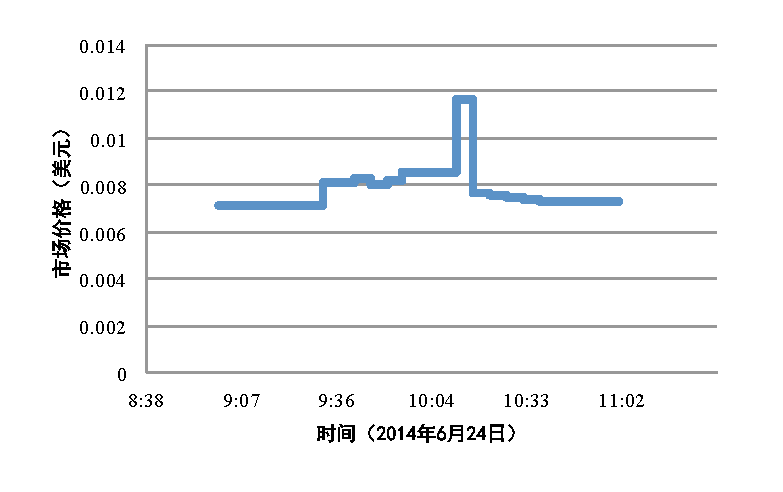
\includegraphics[width=0.9\textwidth]{SpotPrice}
  \caption{一个 us-east-1a 可用区的 linux.m1.small 类型的竞价云实例的市场价格历史数据}
  \label{figure:sil}
\end{figure}

如图 \ref{figure:sil} 所示,竞价云实例市场价格在一段时间 $d_i$ 内保持在一个固定值 $S_{i}$,而后切换到一个新的值 $S_{i+1}$ 。本质上,
市场价格序列 ($S_i, i = 1, 2, \cdots, n$) 和逗留时间序列 ($d_i, i = 1, 2, \cdots, n$) 都可用随机过程来描述. Cohan等人 \cite{chohan2010see} 和 Song 等人 \cite{song2012optimal} 通过验证 Chapman-Kolmogorov 等式 \cite{grimmett1992probability} 证明了竞价云实例的市场价格序列满足马尔可夫性。而其逗留时间序列可以用一个时序点过程 \cite{eltit} 来描述。

由于市场价格之间的逗留时间不满足无记忆性,市场价格的变化可刻画为一个半马尔可夫(semi-Markovian)链模型,Song 等人 \cite{song2012optimal} 在其研究工作中也采用了同样的模型并给出了详细的统计推断。将所有有效市场价格的集合表示为 $\mathcal{S}$,其中 $\mathcal{S} = \{s_i, i = 1, \cdots, \left|\mathcal{S}\right|\}$, 将所有逗留时间的状态空间表示为 $\mathcal{T}$,其中 $\mathcal{T} = \{\tau_i, i = 1, \cdots, \left|\mathcal{T}\right|\}$。该半马尔可夫链的随机核(Stochastic Kernel)可表示为式 \eqref{eq_Q} 。
\begin{equation}\label{eq_Q}
Q(i, j, k) = (q_{i, j, k}; s_i, s_j \in \mathcal{S}, k \in \mathcal{T})
\end{equation}

其中,
\begin{equation}\label{eq_q}
q_{i, j, k} = Pr(S_{n+1} = s_j, S_n = s_i, \tau_n = k)
\end{equation}

式 \eqref{eq_q} 表示状态 $i$ 在时间后 $k$ 转移到状态 $j$ 的概率。

通过这个竞价云实例市场价格模型,我们可以计算未来一段时间两个市场价格间发生转移的概率,进而估计在给定竞价下一个竞价云实例的在未来一段时间的失效概率。

\subsection{成本最优化问题}
竞价决策问题可以抽象为一个非线性规划模型。目标是最小化构建分布式服务的竞价成本。约束是使用竞价云实例部署的分布式服务的可用性不差于使用按需云实例部署的同一服务。分布式服务的可用性估计基于竞价云实例的失效概率。

根据前文介绍的竞价云平台的定价规则,用户无需支付因云平台回收机器造成的不足一小时部分的开销。如果一个用户能够精确估计竞价云实例的价格变化,利用这个特点减少计算成本甚至是零成本计算是可能的。然而,精确预测何时发生价格变化以及变成什么价格是非常困难的。利用竞价不足失效免费使用云计算资源看似美好,实则不太可行。本节无意去探讨利用竞价云平台的这个竞价云实例计费规则来降低成本,以简化使用竞价云实例部署分布式服务的成本最优化问题。

在竞价云平台中,不同的可用区不仅隔离了各种计算实例的硬件、软件错误,而且隔离了竞价不足失效。不同可用区的竞价云实例属于不同的市场。为确保如前文所述申请的竞价云实例节点的失效独立性,分布式服务在每个可用区应该至多申请一个竞价云实例。Amazon EC2 竞价云平台中共有超过 30 个可用区,这对于选出组成一个实际系统中的 Paxos 组(Paxos Group)的节点规模(通常为 5 或 7 个节点)\cite{Burrows:2006:CLS:1298455.1298487} 已经足够。性能需求可通过运行多个并行的 Paxos 组加以满足。

因为竞价云平台一般以小时为单位计费,竞价的周期可设为 $n$ (一个正整数)个小时。在每个竞价周期,成本最小化问题可形式化为一个非线性规划问题。在这个模型中,决策变量是用户在各个可用区给出的竞价。竞价决策可被表示为一个向量 $\bf b$ $= (b_1, b_2, \cdots, b_n)$. 其中,在第$i$个可用区申请竞价云实例的竞价为 $b_i$, $i = 1, 2, \cdots, n$。

当进行竞价时,下一个周期申请到的竞价云实例的开销仍然是未知的。这是因为竞价云平台的计费是以小时为单位结算,而市场价格可能发生变化。对于一个由多个竞价云实例组成的分布式系统,决策目标是各个竞价云实例的成本之和最小。由于未来时间点的竞价云实例市场价格是一个随机变量,我们这里使用竞价云实例的竞价之和作为非线性规划的目标函数。显然竞价之和是实际成本之和的一个上界,通过最小化竞价之和可以严格控制计算成本。

非线性规划模型中的关键约束是确保使用竞价云实例部署的分布式服务有着和使用按需云实例部署的同一服务可用性相当。分布式服务的可用性可被表示为其最优可接受集的可用性。这里将一个分布式服务 $S$ 的最优可接受集表示为 $\mathcal{A}_{o}(S, \bf{FP})$,其中 $\bf{FP}$ 竞价云实例节点失效概率向量。 将一个使用竞价云实例部署的分布式服务表示为 $S_s$, 第 $i$ 个可用区的竞价云实例的市场价格表示为 $p_i$,服务 $S_s$ 中使用的各个可用区的竞价云实例在指定竞价 $\bf b$ =$ (b_1, b_2, \cdots, b_n)$ 下的节点失效概率为 $FP(\bf b)$。类似的,将一个使用按需云实例部署的对应分布式服务表示为 $S_o$,在使用按需云实例部署的服务 $S_o$ 中按需云实例节点个数为 $m$。成本最优化问题最终可形式化为一个非线性规划模型。式 \eqref{eq_min_cost} 为目标函数。
\begin{equation}\label{eq_min_cost}
\min \sum_{i=1}^n b_i
\end{equation}
s.t.
\begin{equation}\label{eq_bgp}
\sum_{i=1}^n {\epsilon(b_i - p_i)} \geq m
\end{equation}

\begin{equation}\label{eq_aae}
A_{\mathcal{A}_{o}(S_o, {\bf{FP^{\prime}}})} - A_{\mathcal{A}_{o}(S_s, FP(\bf b))} < \varepsilon
\end{equation}

其中,不等式 \eqref{eq_bgp} 是一个基本约束,确保开始申请竞价云实例时有足够的节点可用以保证部署的分布式服务能够初始化正确。在不等式 \eqref{eq_aae} 中, $\epsilon$(u) 为一个 $u$ 是否大于0的判定函数,$\varepsilon$ 表示一个无穷小量。在实际使用中,可以将其设置为一个可接受的可用性误差,如 0.000001。

\section{竞价框架及策略}
\label{jupiter-framework}
解决上述非线性规划问题是 NP 难的。需要遍历所有可能的竞价 $\bf b$ 验证其是否满足可用性约束。遍历空间的大小是 $m^n$,其中 $m$ 是可能的价格数,而 $n$ 不同的可用区个数。显然,枚举搜索的方法是无法实际应用的。

既然在可接受的短时间内求得最优解是不可能的,不妨退而求其次获取一个接近最优解的竞价决策。从云租户角度来看,一个竞价决策只要大幅减少竞价云实例的使用成本即可,不一定非要求得最优解。下面主要介绍能够实际应用的成本和可用性感知的使用竞价云实例构建分布式服务的竞价框架。如图 \ref{figure:framework} 所示,竞价决策在每个竞价周期的开始由在线竞价模块给出。然后竞价云实例申请被发送给竞价云平台。竞价云实例失效预测模块用于估计在下一个竞价周期中一个竞价云实例在指定竞价下的失效概率。估计的竞价云实例失效概率用于验证整个分布式服务的可用性需求约束。通过不断收集竞价云实例市场价格数据,竞价云实例的失效概率的预测可以反映市场供需变化。
\begin{figure}
  \centering
  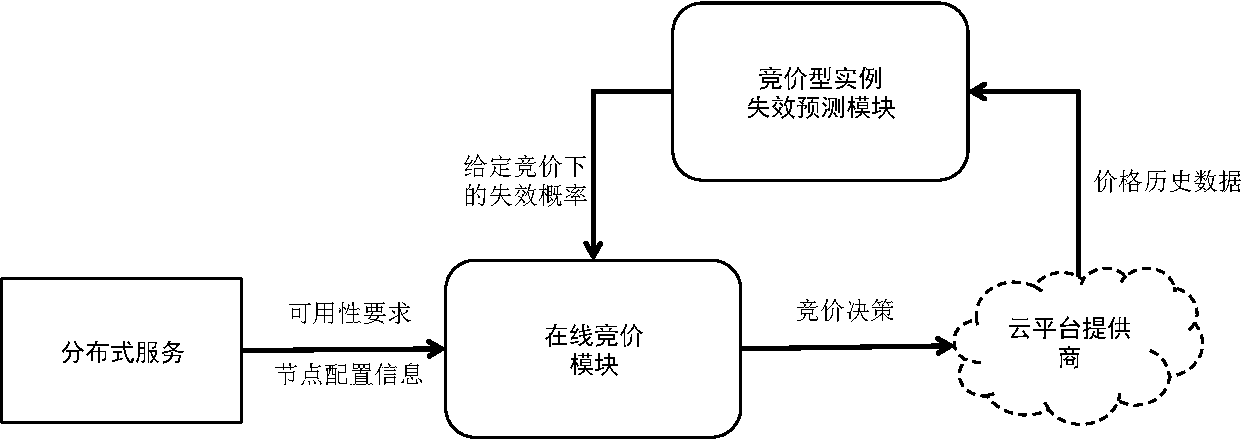
\includegraphics[width=0.85\textwidth]{CAB_arch.pdf}
  \caption{在线竞价框架}
  \label{figure:framework}
\end{figure}

在这个竞价框架下,如果竞价云实例市场价格大幅变动,在新的竞价周期竞价决策将随之发生改变。一些竞价云实例需要被替换为其它可用区的竞价云实例。为保证节点替换过程中服务的可用性,新加入的竞价云实例在新的竞价周期开始之前就被启动并加入到分布式系统中,然后被替换的节点在新的竞价周期开始时被移除。加入和移除竞价云实例可以通过Paxos的视图切换(View Change)操作完成。一个竞价云实例的启动时间通常需要 200 秒或更多,在 Amazon EC2 云平台的不同地理区域有一些差别 \cite{Mao:2012:PSV:2353730.2353859}。因此,每个竞价周期的实际时间由于存在相互覆盖的部分会有所减少。后文中将对不同竞价周期的选取进行讨论。

\subsection{在线竞价算法}
\label{subsec:jupiter-bidding}
如前文所述,在一个传统的分布式系统可用性模型中节点的失效概率是固定的,通常为一个非常小的常数。可行的 Quorum 投票节点组合就是简单的分布式系统中所有节点的大多数。对于分布式系统中的节点失效概率各不相同的情况,往往采用基于权重的投票权分配方法。基于权重的最优可用性投票权分配机制已在 Tong 等人 \cite{25789}、Spasojevic 等人 \cite{262589}、Amir 等人 \cite{Amir1998223} 的工作中得到很好的研究。这里将所有 $n$ 个节点的失效概率表示为 $p_i, i = 1, 2, \cdots, n$。Amir 等人 \cite{Amir1998223} 已经证明:如果 $\forall i, p_i \geq \frac{1}{2}$, 最优投票权分配方式不再是民主式的相同投票权重,而是所有节点中相对可靠性最高的节点拥有绝对权重即由该节点集权。如果系统中只有部分节点 $i$ 满足 $p_i \geq \frac{1}{2}$, 在一个最优投票分配中所有这些失效概率大于 $\frac{1}{2}$ 的节点不应该得到投票权。如果 $\forall i, 0 < p_i < \frac{1}{2}$,最优投票权重可由下式 \cite{262589, 25789} 给出:
\begin{equation}\label{eq_ow}
w_i = log_2(\frac{1-p_i}{p_i})
\end{equation}

然而,在一个实际使用场景中,式 \eqref{eq_ow} 在各个节点失效概率差异较大的情况下不能被直接应用。例如:一个有三个节点的分布式系统中节点失效概率分别是:0.01,0.1,0.1。根据式 \eqref{eq_ow},节点失效概率为0.01的节点拥有占支配地位的投票权,超过了另外两个节点的投票权之和。这在理想情况下是合理的,因为当一个节点的可靠程度远远高于另外两个节点时由它来决定系统可用性是最优的。但在实际情况下,节点的失效概率是在有限时间段内估测出的,与无限时间下平稳态的理想值有一定的偏差。竞价云实例失效模型中的竞价不足失效正是这样一种情况。另外,Paxos系列的协议在设计过程中并未考虑投票权重不同的情况。为保证竞价算法简单性和兼容性,维持 Paxos 组中的简单大多数投票方式是必要的。

由于每个竞价云实例被固定分配了相同的投票权,实现分布式服务的最优可用性要求各个竞价云实例应有相同的失效概率。在本文的在线竞价算法中,各个竞价云实例的失效概率会趋近于相同。该算法使用了枚举和贪心的策略。

\begin{algorithm}
\caption{在线竞价}
\label{algo:bidding}
\KwIn{服务可用性要求 $availability$, 最低节点数限制 $N$}
\KwOut{$bids$}
$zones\gets get\_availability\_zones()$\tcp*[r]{获取所有可用区}
\ForEach{$n \in [N, zones.size]$}
{
  $FP\gets node\_failure\_pr(n, availability)$\tcp*[r]{节点失效概率上限}
  \ForEach{$zone \in zones$}
  {
    \ForEach{$bid \in [zone.spot\_prices[1], zone.on\_demand\_price)$}
    {
      \If{$estimate\_FP(zone, bid, zone.spot\_prices) \not> FP$}
      {
        \textbf{break}\tcp*[r]{给定竞价下估计的失效概率可接受}
      }
    }
    $bids[n][zone]\gets bid$\;
  }
  $sort(bids[n])$\;
  $cost\_upper\_bound[n]\gets sum(bids[n][1:n])$\;
}
$m\gets min\_key(cost\_upper\_bound)$\;
\Return{$bids[m][1:m]$}\;
\end{algorithm}

在线竞价策略如算法 \ref{algo:bidding} 所示。该算法接受一个分布式系统配置信息作为输入,包括系统可用性和节点类型需求等。整个在线竞价算法步骤简单描述如下:1)对于所有可能的节点数 $n$,计算在各个节点失效概率相同情况下的满足系统可用性要求的节点失效概率最大可能值 $FP$。2)在 $n$ 个节点的配置下,对于所有可用区估计失效概率小于 $FP$ 的最小竞价。失效概率的预测依赖于各个可用区的竞价云实例失效概率模型,决定于竞价、竞价云实例市场价格、市场价格逗留时间。3)比较所有可用区的最小竞价值,以贪心的方式选择可用区。4)累加所选择的可用区的最小竞价值,计算在每一个节点数 $n$ 的配置下计算成本的上限并返回成本上限最小的竞价方案作为竞价决策。这个算法不能保证总是给出一个最优的竞价决策,但在实际使用中能给出一个接近最优的竞价方案。

\subsection{失效概率预测}
在整个竞价框架中,在线竞价模块需由竞价云实例失效预测模块完成各个可用区竞价云实例失效概率的预测。为估计竞价云实例的失效概率,竞价云实例的市场价格预测模型被嵌入到竞价云实例失效模型中。如前文中 \ref{jupiter-sifm} 节所述,竞价云实例的市场价格的变化被形式化为一个半马尔可夫链模型。因此,竞价云实例失效概率预测的一个关键任务是从观测到的竞价云实例市场价格历史数据中重新构造出概率转移分布。
研究者Wee\cite{5948651}在2011年认为竞价云实例市场价格采样累计分布函数约每一个小时有明显的增长。然而,新收集到的2014年竞价云实例市场价格数据显示市场价格的变化频率已经加快为每小时多次。简单起见,这里将半马尔可夫链的时间单位设置为1分钟,采样数据中的逗留时间 $d_i$ 被离散化为式 \eqref{eq_tau} 。
\begin{equation}\label{eq_tau}
\tau_i \triangleq \tau(S_i \rightarrow S_{i+1}) \triangleq \lfloor d_i \rfloor
\end{equation}

这里采用一个经验估计方法,本质上类似于极大似然估计(Maximum Likelihood Estimator) \cite{Barbu:2008:SCH:1481376}。统计核(Stochastic Kernel) \textbf{Q} 被重构为式 \eqref{eq_dq} 。
\begin{equation}\label{eq_dq}
\widehat{{q}_{i,j,k}} = \frac{N_{i, j}^{k}}{N_i}, \forall N_i \neq 0
\end{equation}

当$N_i = 0$时,$\widehat{{q}_{i,j,k}} = 0$。

其中,$N_i$ 为价格 $s_i \in \mathcal{S}$在采样历史数据中出现的次数,$N_{i, j}^{k}$ 表示价格在逗留时间 $k \in \mathcal{T}$ 从 $s_i \in \mathcal{S}$ 内转移到价格 $s_j \in \mathcal{S}$ 的次数。

竞价最高可以设置为同类型按需云实例的10倍,当竞价云实例的市场价格高于同配置类型按需云实例时,应选择按需云实例以避免过高的竞价云实例成本。因此,在本文的竞价框架中一个合法的竞价不应超过其对应类型的按需云实例,价格等于对应按需云实例价格的竞价视为申请一个按需云实例。在一个竞价周期,竞价云实例在指定竞价下的失效概率可表示为式 \eqref{eq_fpb} 。
\begin{equation}\label{eq_fpb}
FP(b) = 
\begin{cases}
1 &\mbox{if $0 \leq b \leq p$}\\
1 - (1 - FP^{\prime}) \cdot \sum\limits_{j=p}^b{\widehat{{q}_{p, j, k}}} &\mbox{if p < b < o}
\end{cases}
\end{equation}

其中 $b$ 表示一个竞价,$p$表示竞价云实例市场价格,$k$ 表示逗留时间,$o$ 表示对应类型的按需云实例价格,$FP^{\prime}$ 表示根据 SLA 得到的对应按需云实例的失效概率。

竞价云实例在一个竞价周期的失效概率是其在每个时间单元的失效概率期望,即公式 \eqref{eq_acc_fp} 的离散形式。

\section{系统评测}
\label{sec:jupiter-evaluation}
基于前述竞价框架设计,本章的工作还包括用Python实现了一个面向Amazon EC2云平台的竞价框架原型 \emph{Jupiter}。该竞价框架通过 AWS (Amazon Web Services) 的 Python接口库 \emph{boto} \cite{boto:2014} 同 Amazon EC2 交互。为全面检验 \emph{Jupiter},评测中将其用于在 Amazon EC2 上部署一个分布式锁服务和一个分布式存储服务。整个评测包括一个微基准测试,一个一周时间的运行于 Amazon EC2 的可行性验证测试,和两个11周时间的基于价格历史数据重放的成本和可用性评测。

\subsection{评测涉及的分布式服务}
\label{subsec:jupiter-bc}

\subsubsection{分布式锁服务}
\label{subsection-case-dls}
分布式锁服务一般用于松耦合的分布式系统中。一个代表性的分布式锁服务是 \emph{Chubby} \cite{Burrows:2006:CLS:1298455.1298487},可用于数千个节点的活动同步以及基本信息确认,例如:系统成员信息。

\emph{Chubby} 提供了一个非常像文件系统的建议锁(Advisory Lock)的接口,并使用Paxos作为生产环境下的分布式一致性协议以保证高可用性。一个 \emph{Chubby} 服务端通常配置成5个副本。\emph{Chubby} 客户端通过使用RPC调用库实现和 \emph{Chubby} 服务端的通信。这样五个节点组成的分布式系统的投票方式采用简单多数原则。\emph{Chubby} 遵循不同副本部署于不同区域或数据中心(和 Amazon EC2 等云平台的可用区概念相似)的原则。

\subsubsection{基于纠删码的分布式存储服务}
\label{subsubsec:dss}
分布式存储服务通常为客户端提供对象存储或键值存储,可容忍部分节点的暂时性故障甚至是永久性的机器和磁盘损坏。在多个可用区间构建分布式存储服务可以容忍数据中心故障或网络中断以提供更好的可用性。不同于主从式技术,Gaios \cite{Bolosky:2011:PRS:1972457.1972472} 和 Megastore \cite{baker2011megastore} 已在分布式存储服务的实现中采用了基于 Paxos 的 SMR 机制进行容错。

纠删码 \cite{Rizzo:1997:EEC:263876.263881} 是一种信息理论中的前向错误纠正编码方式,原本用于在网络通信中独立数据包丢失的情况下进行消息恢复,现已广泛用于分布式存储系统 \cite{Huang:2012:ECW:2342821.2342823, Sathiamoorthy:2013:XEN:2488335.2488339},用于减少存储和网络开销。在一个通常形式的纠删码编码中,原始数据通常被划分为$m$个大小相同的数据块,然后计算并生成$k$个大小相同的校验块,数据块的总数是 $n = m + k$。纠删码算法能够从 $n$ 个数据块中的任意 $m$ 个数据块重构出原始数据。这样的一个纠删码编码可以表示为 $\theta (m,n )$。

近来,Mu 等人 \cite{Mu:2014:PME:2600212.2600218} 提出了一个 Paxos 协议的变体,RS-Paxos,可以在异步网络模型下实现分布式系统中基于纠删码的一致性决议。RS-Paxos 可被用于分布式存储系统,通过在各个节点上发送编码后的数据块而不是全部数据拷贝大大减少了网络数据传输和磁盘数据写入。这样的分布式存储服务被称为基于纠删码的分布式服务。

一个标准的 RS-Paxos 配置是 5 个节点,纠删码编码方式为 $\theta(3, 5)$。需要注意的是,这里 RS-Paxos 最多仅能容忍一个节点失效而不是两个节点失效。这和前面讨论的分布式锁服务是非常不同的。这是因为基于纠删码的分布式存储服务中写入操作所需的 Quorum 投票节点数不同于各个节点间数据全副本的方式。为保证能够重构出原始数据,可接受集的交集(Intersection)大小需达到 3,而不是 1。

\subsection{实验设置}
使用按需云实例部署的上述两个分布式服务被设置为后续实验中的基线。虽然使用预留计算实例可以至多减少 30\% $\sim$ 40\% 的成本,由于其不灵活性以及难于适应变化的服务负载,本实验中不再加以比较。根据 Amazon EC2 云平台的文档 \cite{AWS_SLA:2014} ,一个按需云实例的失效概率被设定为 0.01。实验中用到的分布式锁服务是一个基于 Paxos 的简单实现,分布式存储服务是一个基于 RS-Paxos 的实现\cite{Mu:2014:PME:2600212.2600218}。在这两个系统中节点数都配置为 5,这是实际生产系统中的通常配置 \cite{Burrows:2006:CLS:1298455.1298487, Mu:2014:PME:2600212.2600218}。在这样一个配置中,分布式锁服务能够容忍任意不超过两个节点失效,分布式存储服务则只能容忍至多一个节点失效。

实验中使用了一个启发式的竞价策略作为对照组。假设原有使用按需云实例的分布式系统中有 $n$ 个节点,该策略选择竞价云实例市场价格最低的 $n + m$ 个可用区申请竞价云实例,$m$ 为该策略使用的额外节点数。对于每个被选出的可用区,该策略给出的竞价为竞价云实例的市场价格加上一个额外的溢价比例 $p$,如:10\%或20\%。由于有大量的 $m$ 和 $p$ 可供选择,实验中使用了一些有代表性的 $m$ 和 $p$ 用于比较实验结果。方便起见,有 $m$ 个额外节点和超出竞价云实例市场价格比例 $p$ 的启发式策略后文中将表示为 $Extra(m, p)$。

实验中使用了 Amazon EC2 云平台的 17 个可用区。分布式锁服务采用 linux.m1.small 类型实例部署,每个该配置类型按需云实例在各个可用区的价格有所差别,大约为 4.4 $\sim$ 6.1美分/小时。基于纠删码的分布式存储服务使用 linux.m3.large 类型实例构建,该实例类型相比 linux.m1.small 类型拥有更多的计算资源和内存容量。每一个该配置类型按需云实例的价格在各个不同可用区约为 14 $\sim$ 20.1 美分/小时。

对于每一个可用区,竞价云实例失效模型使用大约三个月的竞价云实例市场价格历史数据进行训练。从概率转移矩阵的变化上看,模型已经趋于收敛。在整个评测过程中,我们在 Amazon EC2 云平台上使用竞价框架运行分布式锁服务和基于纠删码的分布式存储服务约一周时间。然后,根据 Amazon EC2 的竞价云实例计费规则重放了两个 11 周长的竞价云实例市场价格数据仿真了前述两个分布式服务在不同竞价框架下的运行。在仿真中,竞价云实例的启动时间已经加以考虑。竞价云实例启动时间在不同区域间有很大不同,通长在 200 $\sim$ 700 秒之间\cite{Mao:2012:PSV:2353730.2353859}。

\subsection{微基准测试}
对于竞价云实例失效预测模块,需要重点关注的是在给定竞价下其对竞价云实例失效概率的预测准确程度。在微基准测试中需要比较测得的竞价云实例失效概率和模型预估的竞价云实例失效概率期望。测试中采用的比较方式为:先使用竞价云实例失效模型确定各个可用区竞价不足失效概率在一个月时间内不超过 0.01 的竞价,然后通过比较竞价和该月的竞价云实例市场价格数据计算实际的竞价不足失效概率。通过比较实际的竞价不足失效概率和 0.01 的差距可以得出竞价云实例失效概率预测的大致可靠程度。图 \ref{figure:fp} 给出了在 5 个可用区的竞价不足失效概率。
\begin{figure}
  \centering
  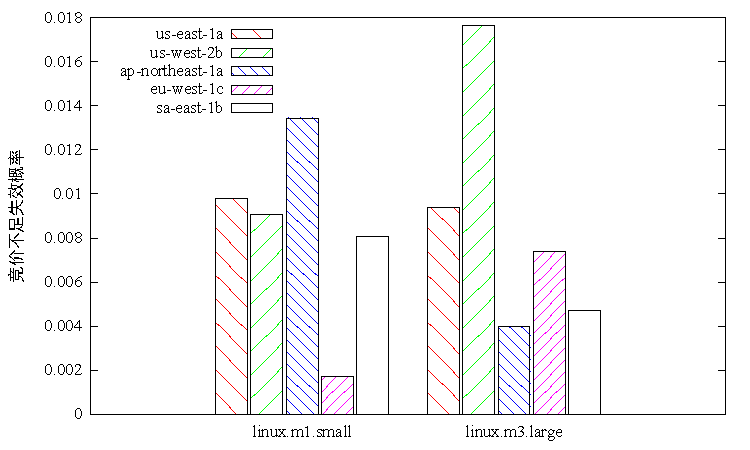
\includegraphics[width=0.9\textwidth]{fp.pdf}
  \caption{预估竞价不足失效概率为 0.01 竞价下的实际失效概率}
  \label{figure:fp}
\end{figure}

对于 linux.m1.small 和 linux.m3.large 两种类型的竞价云实例,大部分情况下测得的竞价不足失效概率都小于0.01。在所有测试中有两个略大于0.01的例外:一个是在 ap-southeast-1a 可用区,针对 linux.m1.small 类型竞价云实例的竞价不足失效概率约为0.013553;另一个是在 us-west-2b 可用区,针对 linux.m3.large 类型的竞价云实例的竞价不足失效概率为0.017665。测试结果表明竞价云实例失效模型可以在一个较小误差内估计失效概率。

\subsection{可行性验证}
在 2014 年 12 月,竞价框架在 Amazon EC2 云平台上进行了长达一周的运行测试。\emph{Jupiter} 竞价框架运行正确,在一周时间内保证了两个分布式服务一直可用。使用 $Extra(0, 0.1)$ 启发式策略的竞价框架作为对照组也同时运行。两个竞价策略中的竞价周期均设为1小时。
\begin{figure}
  \centering
  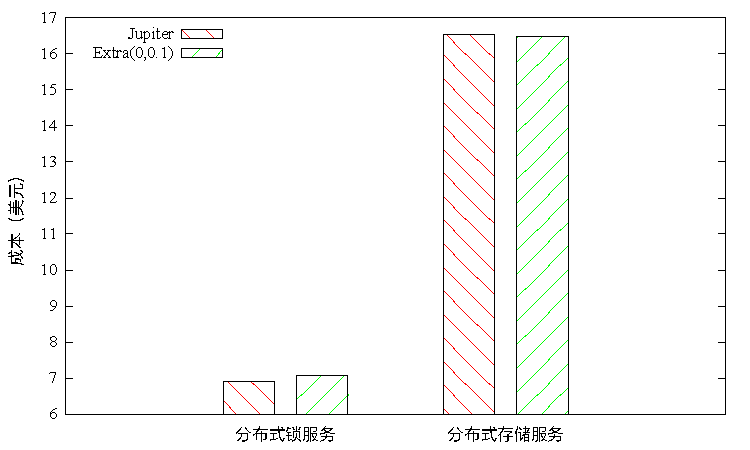
\includegraphics[width=0.85\textwidth]{rr.pdf}
  \caption{不同竞价策略下的竞价云实例成本(2014 年 12 月 15-22 日)}
  \label{figure:rr}
\end{figure}

如图 \ref{figure:rr} 所示,在一周的运行中,\emph{Jupiter} 竞价框架下分布式锁服务的计算成本约为6.91美元,只有使用按需云实例的六分之一左右,也略低于 $Extra(0, 0.1)$ 竞价策略的成本。两个竞价策略在一周的运行中,分布式锁服务一直处于可用状态。相应地,分布式存储服务使用 \emph{Jupiter} 竞价框架运行一周的计算成本是16.53美元,同使用 $Extra(0, 0.1)$ 策略的成本相近。在可用性方面,\emph{Jupiter} 竞价策略保证了分布式存储服务在一周的运行中一直可用,而 $Extra(0, 0.1)$ 策略则出现了一次竞价不足失效导致的服务不可用。总的来看,\emph{Jupiter} 竞价框架在可用性和成本上要好于用于对照的启发式竞价策略。实验结果表明,\emph{Jupiter} 竞价框架是可行的,可在显著减少计算成本的同时保证使用竞价云实例部署的分布式服务高可用。

\subsection{成本和可用性分析}
\label{subsec:ca}
本节通过对长期的竞价云实例市场价格历史数据重放仿真对 \emph{Jupiter} 竞价框架进行评测。因为仿真实验中一个竞价云实例的开销和可用性均由给定的竞价云实例市场价格数据确定,仿真结果同在Amazon EC2平台中运行竞价框架的结果是相同的。两个启发式策略 $Extra(0, 0.2)$ 和 $Extra(2, 0.2)$,也进行了相同的仿真实验作为对照。在仿真实验中,所使用的数据包括2014年10月至12月间的 linux.m1.small 类型和 linux.m3.large 类型竞价云实例的市场价格历史数据。其中,分布式锁服务的仿真实验使用 linux.m1.small 类型竞价云实例的市场价格数据,分布式存储服务的仿真实验采用 linux.m3.large 类型竞价云实例的市场价格数据。评测主要关注两个分布式系统部署案例中服务的可用性和成本。竞价周期除了1个小时外,还测试了其他几种不同的设置。

11 周时间使用 5 个 linux.m1.small 按需云实例的分布式锁服务的计算成本以最便宜的可用区计算是 406.56 美元。对于基于纠删码的分布式存储服务,11 周时间运行 5 个 linux.m3.large 按需云实例以最便宜的可用区计算其成本是 1293.6 美元。这两个值作为成本的评测基线。两个分布式服务在不同竞价策略下的成本如图 \ref{figure:dlscost} 和 \ref{figure:dsscost} 所示。图 \ref{figure:dlsavailability} 和 \ref{figure:dssavailability} 给出了不同竞价策略在可用性方面的评测结果。

如图 \ref{figure:dlscost} 所示,本章提出的竞价策略在分布式锁服务的案例中只需约基线五分之一的成本。将竞价周期设为6小时获得了评测中最好的结果,计算成本约77.3美元。对于1小时,9小时以及12小时的竞价周期,本章提出的竞价策略所需成本略高于对照的启发式策略 $Extra(0, 0.2)$ 。启发式策略 $Extra(2, 0.2)$ 的成本则要明显高于其他两个竞价策略。
\begin{figure}
  \centering
  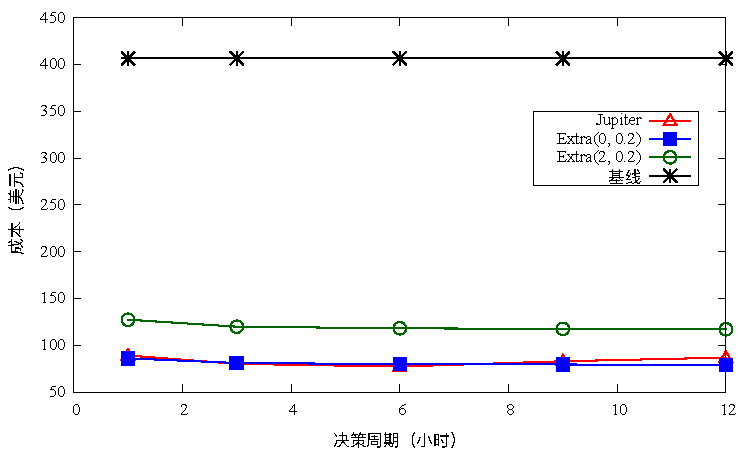
\includegraphics[width=0.9\textwidth]{cost-dls.pdf}
  \caption{不同竞价策略下分布式锁服务的竞价云实例租用成本(2014 年 10-12 月)}
  \label{figure:dlscost}
\end{figure}

对于分布式锁服务的可用性,如图 \ref{figure:dlsavailability} 所示,\emph{Jupiter} 竞价框架几乎没有发生服务失效不可用的情况(可用性和使用按需云实例相当)。而另外两个启发式策略则无法保证相同的可用性级别。在使用对照组启发式策略 $Extra(0, 0.2)$ 时,11周中累计有8小时的时间服务处于故障停机状态。这远远达不到高可用服务的要求。在另外一个对照组启发式策略 $Extra(2, 0.2)$ 下,分布式锁服务的可用性要好于 $Extra(0, 0.2)$ 策略。但在不同竞价周期中仍然无法满足同使用按需云实例相当的服务可用性级别约束。
\begin{figure}
  \centering
  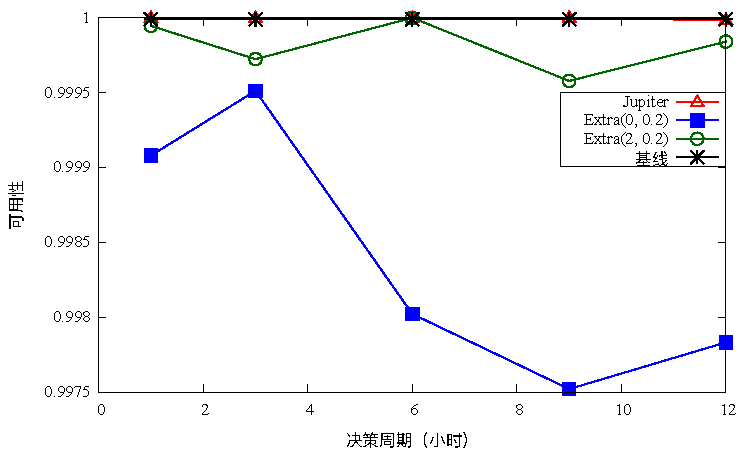
\includegraphics[width=0.9\textwidth]{ava-dls.pdf}
  \caption{不同竞价策略下分布式锁服务的可用性(2014 年 10-12 月)}
  \label{figure:dlsavailability}
\end{figure}

对于策略 $Extra(0, 0.2)$,每个竞价周期申请的竞价云实例数都是5个。而策略 $Extra(2, 0.2)$ 每次申请的竞价云实例数都是7个。策略 $Extra(2, 0.2)$ 在服务可用性方面显然在所有情况下都要好于策略 $Extra(0, 0.2)$。评测结果表明:在没有对竞价云实例失效概率预估的情况下很难有效保证服务可用性级别,即使增加额外的竞价云实例可以一定程度上提高分布式服务的可用性。另外, $Extra(2, 0.2)$ 策略为两个增加的节点花费了31 $\sim$ 41美元的额外成本。 \emph{Jupiter} 竞价框架在可用性和成本两个方面都要优于这两个启发式竞价策略。

对于分布式存储服务,图 \ref{figure:dsscost} 展示了  \emph{Jupiter}  竞价框架在不同竞价周期下所需要的成本。最好的情况还是竞价周期为6小时的配置,分布式存储服务在11周时间里所需成本为189.93美元。相比使用按需云实例,计算成本削减了超过1000美元。在对照组策略 $Extra(0, 0.2)$ 中,所需成本平均为183.5美元。这要略微低于  \emph{Jupiter}  竞价框架的成本,主要原因是在策略 $Extra(0, 0.2)$ 下竞价云实例发生了非常多的竞价不足失效而使得所需支付的计算成本减小。
\begin{figure}
  \centering
  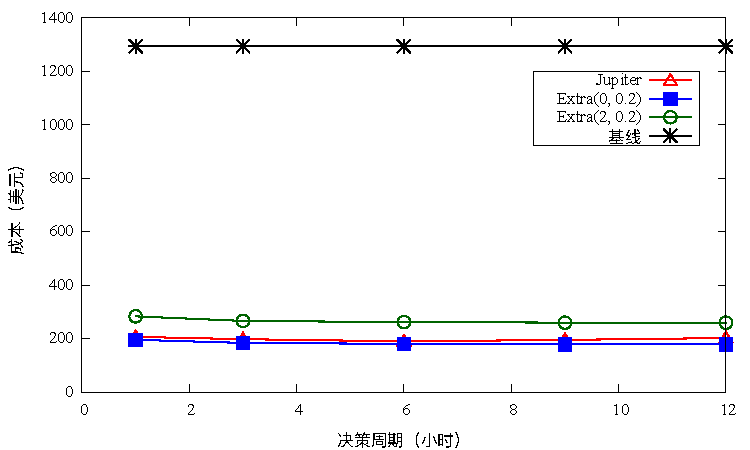
\includegraphics[width=0.9\textwidth]{cost-dss.pdf}
  \caption{不同竞价策略下基于纠删码的分布式存储服务的竞价云实例租用成本(2014 年 10-12 月)}
  \label{figure:dsscost}
\end{figure}

\emph{Jupiter} 竞价框架除竞价周期为 9 个小时的配置均保证了和基线相当的服务可用性级别。在竞价周期为 9 个小时的配置下,分布式存储服务的失效时间略长于可用性级别的要求。与之相比,启发式策略 $Extra(0, 0.2)$ 虽成本略低但服务的可用性级别完全处于不可接受的程度。而启发式策略 $Extra(2, 0.2)$ 虽然在可用性相比 $Extra(0, 0.2)$ 策略有所改善,接近 \emph{Jupiter}  的竞价策略。但 $Extra(2, 0.2)$ 策略所需成本远远高于 \emph{Jupiter} 的竞价策略。详细评测结果参见图 \ref{figure:dsscost} 和 \ref{figure:dssavailability}。
\begin{figure}
  \centering
  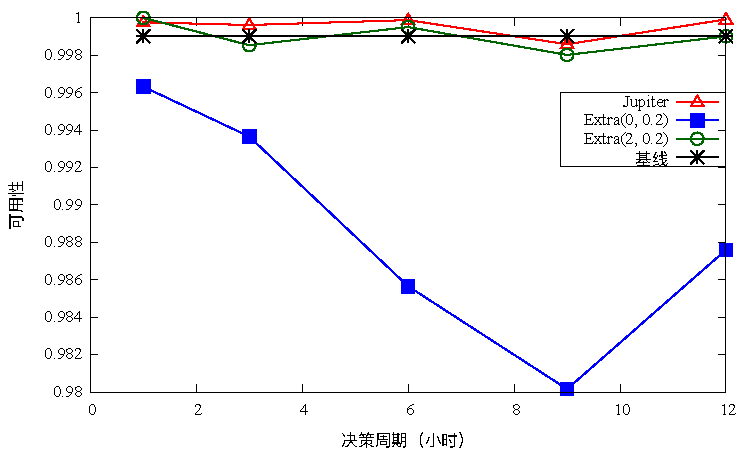
\includegraphics[width=0.9\textwidth]{ava-dss.pdf}
  \caption{不同竞价策略下基于纠删码的分布式存储服务的可用性(2014 年 10-12 月)}
  \label{figure:dssavailability}
\end{figure}

在图\ref{figure:dlscost} 和 \ref{figure:dsscost}中,本文提出的竞价框架所需成本随不同的竞价周期变动很大。一个短的竞价周期意味着更频繁的申请、切换新的竞价云实例会带来很多的竞价周期重叠,减少了有效的运行时间增加了计算成本。然而一个很长的竞价周期设置下则失去了一些根据市场价格变化改变竞价的机会,因为出于保证服务可用性的考虑在一个较长的竞价周期,竞价框架给出的竞价会更高。6 小时的竞价周期设置是几个竞价周期中表现最好的。针对 \emph{Jupiter} 竞价框架的一个扩展是检测竞价云实例市场价格大幅波动的频率并针对性地调整竞价周期。

评测中用于对照的启发式策略是简单和固化的。在没有各个可用区竞价云实例市场价格历史数据知识的情况下,笼统的在市场价格基础上增加一个相同的比例作为竞价是过于粗放的。另外,这样的策略由于没有对竞价云实例失效概率的估计也无法保证分布式服务的可用性级别。额外的新增竞价云实例和一定程度的溢价比例减少了潜在的服务失效,但也显著的增加了成本。总之,这类简单易行的方法不能同时大量节省成本并保证服务的可用性。而 \emph{Jupiter} 竞价框架则可以做到成本和可用性感知,在保证可用性的同时大大减少了计算成本。

\section{本章小节}
\label{sec:jupiter-conclusion}
本章力图解决使用云平台中的竞价云实例构建分布式服务时如何通过竞价决策保证服务可用性的问题。文中指出了使用竞价云实例时保证分布式系统可用性级别面临的挑战,系统可用性的分析因为竞价云实例失效模型的不同而变得复杂。竞价不足失效是竞价云实例的主要失效原因,这完全不同于传统分布式系统中的节点失效。为预测竞价云实例的失效概率,文中引入了半马尔可夫链模型来描述竞价云实例市场价格的变动。使用竞价云实例的分布式系统的可用性期望据此可通过节点失效概率估测,而不是用可同时容忍的最多失效节点数表示。通过竞价决策保证可用性的问题进而被形式化为一个非线性规划问题。优化目标是最小化使用竞价云实例的成本,关键约束表达了分布式服务的可用性要求。然而,解这样一个非线性规划问题是 NP 难的。类似穷举搜索的方法完全无法在实际情况中使用。

本章设计了一个用于在云平台中使用竞价云实例部署高可用分布式服务的竞价框架 \emph{Jupiter},并提出了一个可用于实际生产环境的接近最优解的基于枚举和贪心策略的竞价算法。最后食用两个基础的分布式服务,分布式锁服务和基于纠删码的分布式存储服务验证竞价框架的有效性。\emph{Jupiter} 竞价框架针对分布式锁服务和分布式存储服务在保证同使用按需云实例部署的同一服务具有相同的可用性级别的前提下,可减少81.23\% 和 85.32\% 的计算成本。
